%!TEX root = main.tex
%%%%%%%%%%%%%%%%%%%%%%%%%%%%%%%%%%%%%%%%%%%%%%%%%%%%%%%%%%%%%%%%%%%%%%%%%%%%%%%%

\section{Results}
\label{sec:results}


\begin{figure}[t]
\centering
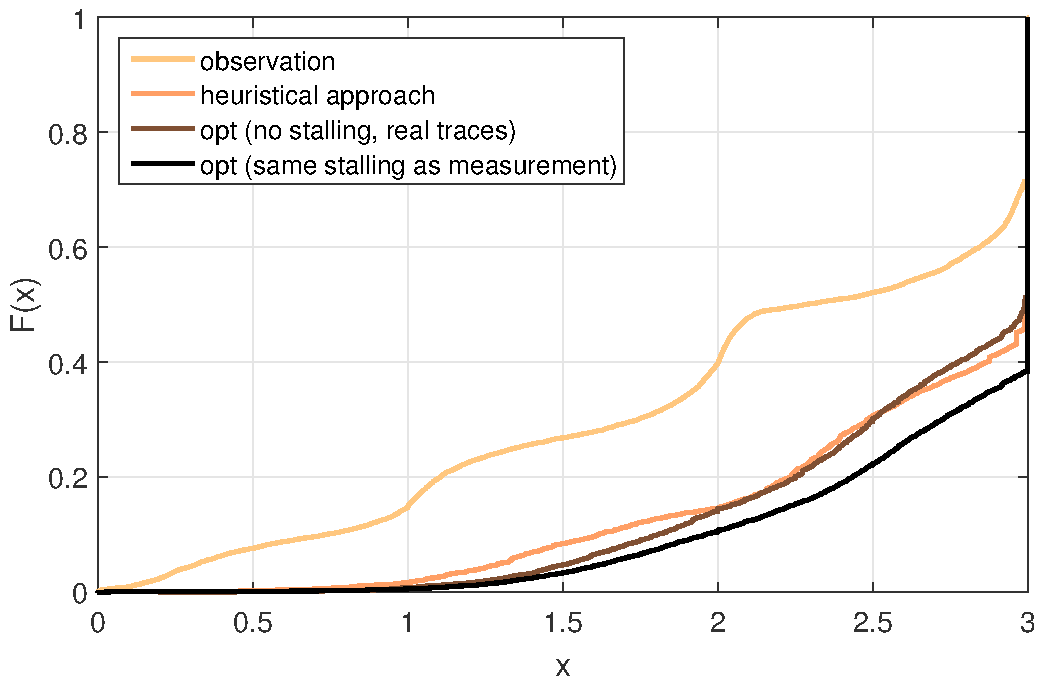
\includegraphics[width=0.5\textwidth]{figs/quality}%
\caption{CDF of the mean video quality in the measurement runs and highest achievable mean video quality according to the optimization problem [REF to opt problem needed]. Remake figure!}
\label{fig:opt}%
\end{figure}


In figure \ref{fig:opt} we see the CDF of the mean video quality in the measurement runs and highest achievable mean video quality according to the optimization problem. In addition, we added an estimation of the avg. quality level that is possible based on downloaded data that was done in [BIEBnetworking2016]. While stalling events occured frequently during the original measurement, stalling events are not allowed to occur in the optimization problem. Therefore, we consider two sets of input for the opt. prob. for each measurement run: First, we consider the duration of the video down...